%========================================================
\chapter{Design of the Proposed TBML Detection Framework}
%========================================================

This chapter presents the design of the proposed \gls{tbml} detection framework. It brings together the software requirements, overall architecture, and module-level design, then walks through the operational requirements and user roles, the system workflows, graph-construction approach, federated learning setup, data-flow representations, and the analytical modules used for detection, investigation, and reporting.

% =====================================
\section{Software Requirements Specifications}
% ========================================================

The software requirements for the proposed TBML detection framework describe what the system needs in order to operate reliably in a real institutional setting. They cover the functional behavior of the platform, the quality attributes it must maintain, the software stack it depends on, and the hardware resources needed to support fraud analysis, transaction monitoring, secure access, and compliance management. The details are grouped into functional requirements, non-functional requirements, software requirements, and hardware requirements in the following subsections.
%========================================================
\subsection[Overall Description]{\textbf{Overall Description}}
%========================================================

The proposed framework is built as a privacy-preserving financial monitoring platform for identifying suspicious Trade-Based Money Laundering activity across large-scale transactional ecosystems. It combines heterogeneous graph-learning mechanisms, federated analytical workflows, role-based monitoring dashboards, and automated Suspicious Transaction Report (STR) generation within a centralized compliance-monitoring environment. In practice, the framework supports real-time transaction monitoring, graph-based fraud classification, institutional investigation workflows, and regulator-side analytical visualization for exposing hidden laundering relationships across connected financial networks.

%========================================================
\subsubsection[Product Perspective]{\textbf{Product Perspective}}
%========================================================
The proposed TBML detection framework acts as a financial monitoring and fraud-analysis platform that brings heterogeneous graph modeling, Graph Neural Network-based analytics, federated learning, and compliance monitoring into one environment. It represents financial entities such as accounts, organizations, invoices, and transactions as connected graph structures so that hidden relationships and suspicious laundering patterns can be captured more effectively than with conventional rule-based Anti-Money Laundering systems. Role-based dashboards are also included to support transaction monitoring, fraud review, alert management, and automated Suspicious Transaction Report (STR) generation.
%========================================================
\subsubsection[Product Functions]{\textbf{Product Functions}}
%========================================================

The primary functionalities supported by the proposed framework are summarized as follows:

\begin{itemize}

\item \textbf{Transaction Monitoring:}  
The system continuously monitors financial transactions and trade-related activities to identify suspicious transactional behavior within large-scale financial ecosystems.

\item \textbf{Graph-Based Financial Analysis:}  
Financial entities such as accounts, organizations, invoices, and transactions are represented as interconnected graph structures for relational analysis and hidden dependency detection.

\item \textbf{Fraud Classification and Risk Prediction:}  
Graph Neural Network-based analytical models classify suspicious transactions and generate fraud risk predictions based on transactional relationships and behavioral patterns.

\item \textbf{Federated Learning Support:}  
The framework supports collaborative model training across multiple institutional environments while preserving sensitive financial data privacy.

\item \textbf{Real-Time Dashboard Visualization:}  
Interactive monitoring dashboards provide visualization of transaction analytics, fraud alerts, risk distributions, and suspicious activity summaries for compliance analysts.

\item \textbf{Suspicious Transaction Report (STR) Generation:}  
The system automatically generates structured Suspicious Transaction Reports for identified fraudulent transactions to support compliance and regulatory workflows.

\item \textbf{Authentication and Role-Based Access Control:}  
Secure authentication and controlled access mechanisms are incorporated to manage user privileges and protect sensitive financial information within the monitoring platform.

\end{itemize}


%========================================================
\subsubsection[User Characteristics]{\textbf{User Characteristics}}
%========================================================

The proposed TBML detection framework supports multiple categories of institutional users involved in fraud monitoring, compliance verification, and regulatory supervision activities. Since the system processes sensitive transactional and compliance-related information, role-based access mechanisms are enforced to ensure secure and controlled interaction with the platform. The major user categories associated with the proposed framework are summarized as follows:

\begin{itemize}

\item \textbf{Bank Compliance Team:}  
The bank compliance team represents institutional analysts responsible for monitoring transactional activities and investigating suspicious financial behavior identified by the fraud-detection framework. These users are expected to possess domain knowledge related to Anti-Money Laundering (AML) procedures, transaction analysis, and institutional compliance operations. Authorized compliance personnel interact with analytical dashboards, review suspicious transaction records, verify fraud alerts, and manage institutional STR escalation workflows.

\item \textbf{Regulatory Administrator:}  
The regulatory administrator functions as a supervisory authority responsible for overseeing fraud-monitoring activities across participating financial institutions. These users typically possess advanced regulatory and compliance expertise associated with financial investigation and institutional auditing operations. Regulatory administrators access consolidated Suspicious Transaction Reports (STRs), monitor institution-level compliance activities, and supervise large-scale suspicious transactional behavior across distributed banking environments.

\end{itemize}




%========================================================
\subsubsection[Constraints]{\textbf{Constraints}}
%========================================================

The development and deployment of the proposed TBML detection framework are subject to multiple operational, computational, and regulatory constraints associated with financial monitoring systems. These limitations influence the scalability, analytical performance, and real-time operational capabilities of the framework.

The major constraints associated with the proposed system are summarized as follows:

\begin{itemize}

\item \textbf{Data Privacy and Regulatory Constraints:}  
Financial institutions operate under strict privacy regulations and compliance policies that restrict direct sharing of sensitive transactional information across organizations.

\item \textbf{Large-Scale Transactional Data Processing:}  
The system must process large volumes of interconnected financial transactions and graph relationships, which may increase computational complexity and memory utilization during real-time analysis.

\item \textbf{Availability of Real-World TBML Datasets:}  
Access to publicly available Trade-Based Money Laundering datasets is limited due to confidentiality and regulatory restrictions, making large-scale real-world experimentation challenging.

\item \textbf{Dynamic Fraud Patterns:}  
Money laundering strategies continuously evolve over time, requiring fraud detection models to adapt to changing transactional behaviors and emerging laundering techniques.

\item \textbf{Infrastructure and Computational Limitations:}  
Training graph-based machine learning models and processing heterogeneous financial networks require significant computational resources, especially for large-scale transactional ecosystems.

\end{itemize}

%========================================================
\subsection[Specific Requirements]{\textbf{Specific Requirements}}
%========================================================

The specific requirements define the operational behavior, performance expectations, software dependencies, and computational resources needed for the framework to run efficiently. They make sure the system can support real-time fraud analysis, scalable monitoring, secure interaction, and intelligent compliance management within financial institutions.

%========================================================
\subsubsection[Functional Requirements]{\textbf{Functional Requirements}}
%========================================================

The functional requirements define the major operations and services that must be supported by the proposed TBML detection framework. The primary functional requirements of the system are summarized as follows:


\begin{itemize}


\item The system shall enforce role-based authorization policies to regulate operational access privileges for compliance analysts and regulatory administrators.

\item The framework shall support ingestion and preprocessing of transactional datasets for heterogeneous financial graph construction.

\item The proposed system shall model financial entities, transactions, and trade relationships as interconnected heterogeneous graph structures.

\item The analytical engine shall perform graph-based fraud classification and generate transaction-level risk predictions using federated learning methodologies.

\item The dashboard infrastructure shall support real-time visualization of suspicious transactions, fraud alerts, analytical summaries, and compliance-monitoring activities.

\item The system shall enable institutional compliance teams to review suspicious transactions and perform fraud escalation or clearance procedures.

\item The framework shall provide features to generate Suspicious Transaction Reports (STRs) for transactions identified as potentially fraudulent.

\item The regulator-side monitoring interface shall support centralized supervision of institutional fraud reports and suspicious financial activities.

\item The analytical interface shall provide transaction-filtering, search, and investigative querying functionalities for fraud-analysis workflows.


\end{itemize}





%========================================================
\subsubsection[Non-Functional Requirements]{\textbf{Non-Functional Requirements}}
%========================================================

The non-functional requirements define the quality attributes, operational constraints, and performance expectations associated with the proposed TBML detection framework. These requirements ensure that the system remains scalable, secure, reliable, and responsive while processing large-scale financial transactions and analytical workloads.

The primary non-functional requirements associated with the proposed system are summarized as follows:

\begin{itemize}

\item \textbf{Scalability:}  
The framework should support scalable processing of large transactional datasets and heterogeneous graph structures without significant degradation in analytical performance.

\item \textbf{Real-Time Processing:}  
The system should support low-latency transaction analysis and fraud prediction to enable continuous real-time monitoring of suspicious financial activities.

\item \textbf{Security and Privacy:}  
The framework should ensure secure access control, protected communication, and privacy-preserving handling of sensitive financial information and compliance-related data.

\item \textbf{Reliability:}  
The system should maintain stable analytical performance and continuous monitoring capabilities during prolonged operational workloads and concurrent user access.

\item \textbf{Availability:}  
The monitoring platform should provide consistent access to dashboards, fraud analytics, and reporting services for authorized institutional users.

\item \textbf{Maintainability:}  
The system architecture should support modular development, efficient debugging, and simplified integration of additional analytical modules and monitoring functionalities.

\item \textbf{Usability:}  
The dashboard interfaces and visualization systems should provide intuitive interaction mechanisms for compliance analysts and regulatory administrators during fraud investigation activities.

\end{itemize}


%========================================================
\subsubsection[Software Requirements]{\textbf{Software Requirements}}
%========================================================

The implementation of the proposed TBML detection framework depends on a combination of software technologies, machine learning libraries, backend services, database systems, and visualization tools. Together, these components support graph-based fraud detection, federated learning, real-time transaction monitoring, and compliance management. The framework therefore needs coordinated interaction between the frontend dashboard, backend processing services, database layers, and machine learning environments. The software requirements are summarized in Table~\ref{tab:software_requirements}.
\vspace{0.3cm}

\footnotesize
\renewcommand{\arraystretch}{1.5}

\begin{table}[H]

\caption{Software Requirements of the Proposed TBML Detection Framework}
\label{tab:software_requirements}

\vspace{0.2cm}

\centering

\begin{tabular}{|p{3.5cm}|p{4.2cm}|p{5.8cm}|}

\hline
\textbf{Category} & \textbf{Technologies / Tools} & \textbf{Purpose in the System} \\
\hline

Operating System 
& Windows 11 
& Provides the development and deployment environment for backend services, databases, and analytical modules. \\
\hline

Programming Languages 
& Python, JavaScript 
& Used for backend development, machine learning workflows, API services, and frontend application development. \\
\hline

Frontend Frameworks 
& Next.js, React.js, Tailwind CSS 
& Supports responsive user interface development, dashboard visualization, and real-time monitoring functionalities. \\
\hline

Backend Framework 
& FastAPI 
& Facilitates asynchronous API communication between frontend dashboards and backend fraud detection services. \\
\hline

Database Systems 
& PostgreSQL, Memgraph 
& Stores transactional records, graph relationships, compliance information, and analytical data required for fraud analysis. \\
\hline

Machine Learning Frameworks 
& PyTorch, PyTorch Geometric 
& Supports deep learning operations, Graph Neural Network implementation, and graph-driven fraud analysis. \\
\hline

Federated Learning Framework 
& Flower 
& Enables distributed federated learning and privacy-preserving model aggregation across institutional environments. \\
\hline

Streaming Platform 
& Apache Kafka 
& Supports real-time transaction streaming and event-driven processing within the monitoring pipeline. \\
\hline

Containerization Platform 
& Docker 
& Provides containerized deployment and scalable execution environments for system integration. \\
\hline

LLM Integration Service 
& Groq LLM API 
& Supports automated generation of Suspicious Transaction Reports and compliance-oriented analytical summaries. \\
\hline

\end{tabular}

\end{table}

\normalsize
%========================================================
\subsubsection[Hardware Requirements]{\textbf{Hardware Requirements}}
%========================================================

The implementation of the proposed TBML detection framework also needs a defined hardware setup to support graph processing, machine learning execution, federated coordination, real-time transaction monitoring, and dashboard visualization. The required hardware is summarized in Table~\ref{tab:hardware_requirements}.

\vspace{0.3cm}

\footnotesize
\renewcommand{\arraystretch}{1.4}

\begin{table}[H]


\caption{Hardware Requirements of the Proposed TBML Detection Framework}
\label{tab:hardware_requirements}

\vspace{0.2cm}

\centering

\begin{tabular}{|p{3.0cm}|p{2.6cm}|p{8.0cm}|}

\hline
\textbf{Hardware Component} & \textbf{Minimum Requirement} & \textbf{Purpose in the System} \\
\hline

Processor & Intel Core i7 / AMD Ryzen 7 & Supports efficient execution of graph analytical models, backend services, and machine learning computations. \\
\hline

RAM & 16 GB & Supports graph datasets, real-time analytical workloads, and concurrent monitoring operations. \\
\hline

GPU & NVIDIA RTX 3050 & Accelerates Graph Neural Network training and deep learning computations. \\
\hline

Storage & 512 GB SSD & Stores transactional datasets, graph databases, analytical models, and generated compliance reports. \\
\hline


\end{tabular}

\end{table}

\normalsize

%========================================================
\section{High level Design}
%========================================================

This section outlines the high-level design of the proposed TBML detection framework. It covers the main architectural choices, the design considerations behind them, and the overall system layout that brings graph-based fraud detection, federated learning, and real-time monitoring together in a single compliance platform.
%========================================================
\subsection[Design Considerations]{\textbf{Design Considerations}}
%========================================================

The design of the proposed TBML detection framework is shaped by operational, analytical, and security requirements that are common in large-scale financial monitoring systems. Because Trade-Based Money Laundering involves connected financial entities, cross-border transactions, and hidden transactional dependencies, the architecture has to support scalable analytical processing, secure institutional collaboration, and efficient graph-based fraud analysis. The major design considerations are discussed in the following subsections.

%========================================================
\subsubsection[General Considerations]{\textbf{General Considerations}}
%========================================================

The proposed TBML detection framework is designed to support large-scale transaction monitoring and fraud analysis across distributed financial environments. Since laundering activities typically involve interconnected accounts, trade entities, invoices, and transactional relationships, the framework uses graph-based modeling to represent hidden financial dependencies more effectively than conventional relational systems. The architecture also supports real-time transaction processing and scalable analytical workflows as institutional transaction volumes continue to grow.

Security, privacy preservation, and scalability are central concerns in the proposed architecture because of the sensitive nature of financial and compliance data. To address them, the framework uses secure authentication, role-based access control, and federated learning so institutions can collaborate without sharing raw transactional data. The system is also built with a modular structure to make integration, maintenance, and future extension of monitoring, fraud detection, compliance reporting, and visualization services easier.


%========================================================
\subsubsection[Development Methods]{\textbf{Development Methods}}
%========================================================

The proposed TBML detection framework is developed using a modular and iterative approach so that the system can be integrated cleanly and its analytical functions refined step by step. Individual components such as transaction monitoring, graph construction, fraud detection, federated learning, and dashboard interfaces are built and tested separately before being brought together in the full monitoring framework.

The development process also includes incremental model evaluation and experimentation to improve fraud detection performance and analytical reliability. Graph-based machine learning models are trained on processed transactional datasets, while frontend and backend services are connected through API-based communication to support real-time interaction between monitoring modules and analytical services.

Version control and collaborative development practices are used throughout the implementation process to manage backend services, machine learning workflows, frontend interfaces, and analytical settings efficiently. This modular approach also makes debugging, testing, maintenance, and future enhancement much more manageable.

%========================================================
\subsection[Architectural Strategies]{\textbf{Architectural Strategies}}
%========================================================

The architectural strategies adopted in the proposed TBML detection framework are aimed at supporting scalable financial transaction analysis, secure institutional collaboration, and smooth interaction between analytical services and monitoring interfaces. The framework brings graph-based fraud detection models, backend analytical services, real-time dashboards, and distributed learning mechanisms together in a unified monitoring environment. The main architectural strategies are discussed in the following subsections.


%========================================================
\subsubsection[Programming Language]{\textbf{Programming Language}}
%========================================================

The proposed TBML detection framework primarily uses Python for backend services, graph processing, machine learning workflows, and analytical computation. Python was chosen because it has strong support for deep learning libraries, graph analytical frameworks, and federated learning environments. Libraries such as PyTorch, PyTorch Geometric, and Flower are used to implement the graph neural network models and distributed learning mechanisms within the fraud detection framework.

The frontend monitoring dashboard is developed using Next.js and React.js to support responsive user interface design and real-time analytical visualization. JavaScript and TypeScript are used to implement dashboard components, transaction monitoring interfaces, and compliance management services. FastAPI is also integrated to support API-based communication between frontend dashboards, backend services, and machine learning modules.


%========================================================
\subsubsection[System Integration Architecture]{\textbf{System Integration Architecture}}
%========================================================

The proposed framework follows a modular client-server and service-oriented integration architecture so that the analytical modules, backend services, and frontend monitoring interfaces can work together in a coordinated way. The fraud detection models, transaction monitoring services, authentication modules, and compliance reporting components operate as independent services while staying synchronized through backend APIs and shared database environments.

The machine learning modules responsible for graph processing and fraud prediction run separately from the frontend monitoring dashboard. Processed fraud predictions, transaction classifications, and generated Suspicious Transaction Reports are synchronized through backend services so that the dashboard can display them in real time and support compliance management. This modular integration approach makes the framework easier to scale, maintain, and extend.


%========================================================
\subsubsection[Data Storage Management]{\textbf{Data Storage Management}}
%========================================================

The proposed TBML detection framework uses both relational and graph-based database systems to manage financial data efficiently and support analytical processing. Structured transactional records, authentication information, compliance-related data, and generated Suspicious Transaction Reports are stored in PostgreSQL. This relational database layer provides secure storage and efficient retrieval of operational monitoring data for the framework.

For the graph database environment, Memgraph is used to store the connected financial entities and transactional relationships. Graph nodes and edges represent accounts, organizations, invoices, and transactions for relational fraud analysis and graph neural network processing. Using relational and graph storage together improves scalability, analytical flexibility, and synchronization between backend analytical services and monitoring dashboards.
%========================================================
\subsection[Overall System Architecture]{\textbf{Overall System Architecture}}
%========================================================
The proposed TBML detection framework combines transaction processing, heterogeneous graph construction, federated learning, and graph-based fraud analytics within a single monitoring environment. Transaction records, trade documents, KYC information, and institutional logs are processed and transformed into heterogeneous financial graphs that capture relationships among accounts, organizations, invoices, and transactions. These graph representations are then analyzed using a hybrid HGNN--LSTM architecture to learn structural dependencies and temporal transaction behavior associated with laundering activity.

To support privacy-preserving collaboration, participating institutions train locally and share only model updates through the federated learning environment. The aggregated global model is then used for transaction risk scoring, fraud classification, and compliance monitoring. High-risk transactions are forwarded to compliance-management services for alert generation, Suspicious Transaction Report (STR) creation, and regulator-side monitoring. The overall architecture of the proposed framework is illustrated in Figure~\ref{fig:overall_architecture}.

\begin{figure}[H]
    \centering
    \fbox{
        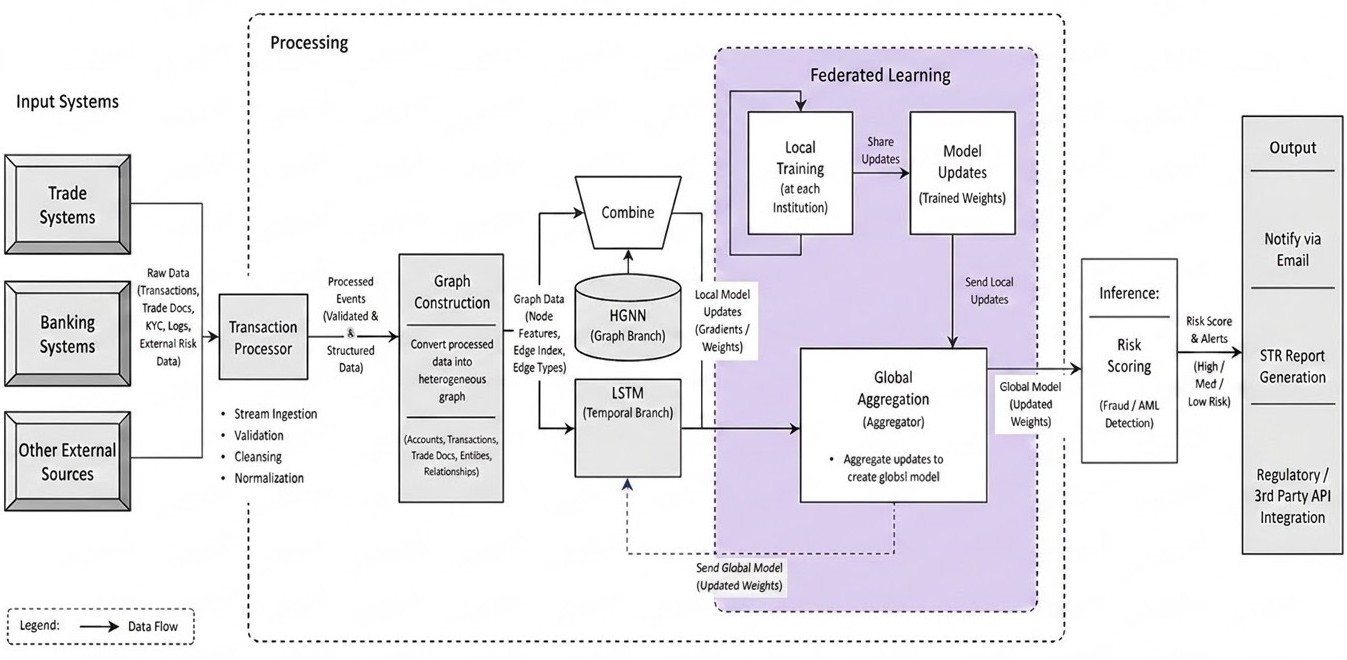
\includegraphics[width=0.98\textwidth]{Figures/overall_architecture.jpg}
    }
    \caption{Overall Architecture of the Proposed TBML Detection Framework}
    \label{fig:overall_architecture}
\end{figure}

%========================================================
\subsection[Data Flow Diagrams]{\textbf{Data Flow Diagrams}}
%========================================================

A Data Flow Diagram (DFD) is a simple way to show how data moves through a system and how processes, external entities, and data repositories relate to one another. DFDs make it easier to see how information enters the system, gets processed, is stored, and then moves to other components. In the proposed Federated Heterogeneous Graph Neural Network (HGNN)-Based Trade-Based Money Laundering (TBML) Detection System, they are used to represent transaction acquisition, graph construction, federated learning, fraud analysis, and alert generation. The split into Level 0, Level 1, and Level 2 diagrams gives a clearer view of the operational flow, the subsystem interactions, and the data-processing steps involved in real-time AML analytics. The diagrams follow the Yourdon and De Marco DFD methodology for consistency.

%========================================================
\subsubsection[Data Flow Diagram Level 0]{\textbf{Data Flow Diagram Level 0}}
%========================================================

\begin{figure}[H]
    \centering
    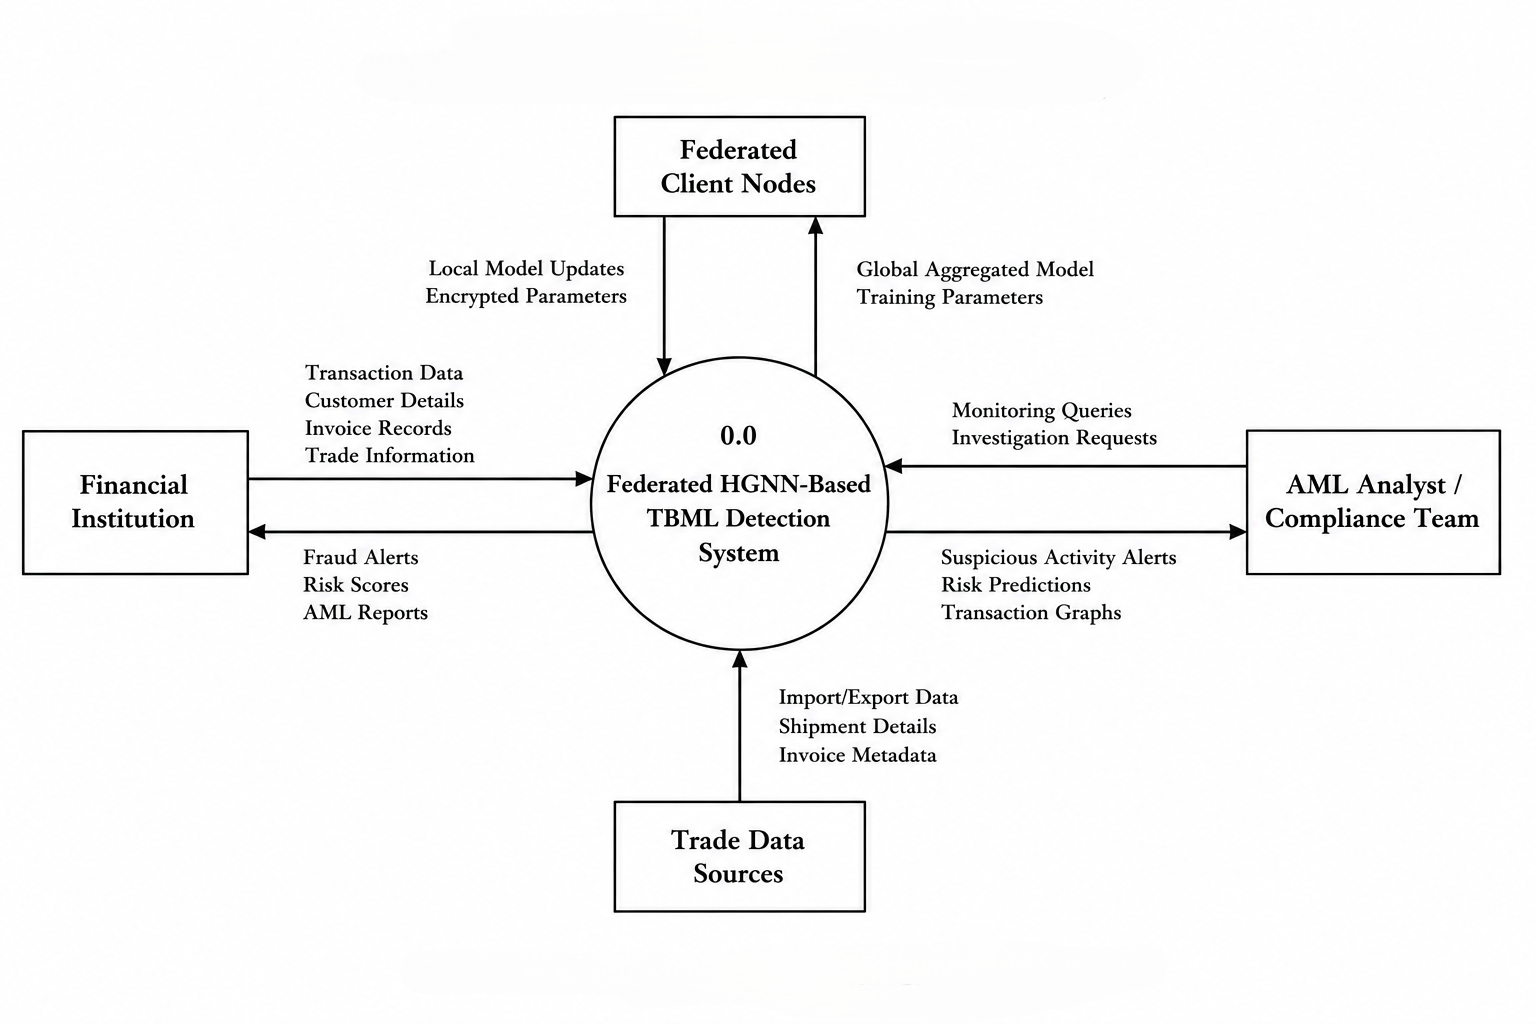
\includegraphics[width=0.95\linewidth]{Figures/DFD_Level_0.png}
    \caption{Level 0 Data Flow Diagram}
    \label{fig:dfd_level0}
\end{figure}

The Level 0 Data Flow Diagram (DFD) of the designed Federated HGNN-Based TBML Detection System is shown in Figure \ref{fig:dfd_level0}. It gives a top-level view of the system as a single process interacting with external entities such as Financial Institutions, Federated Client Nodes, AML Analysts, and Trade Data Sources. The system receives transaction records, customer information, invoice details, and trade details from financial institutions, while trade data sources contribute import/export records and shipment data that help validate transactions and support graph construction. Federated client nodes exchange encrypted local model parameters with the global model, and the system produces fraud warnings, risk assessments, AML reports, and suspicious activity notifications for analysts and compliance teams.

%========================================================
\subsubsection[Data Flow Diagram Level 1]{\textbf{Data Flow Diagram Level 1}}
%========================================================

\begin{figure}[H]
    \centering
    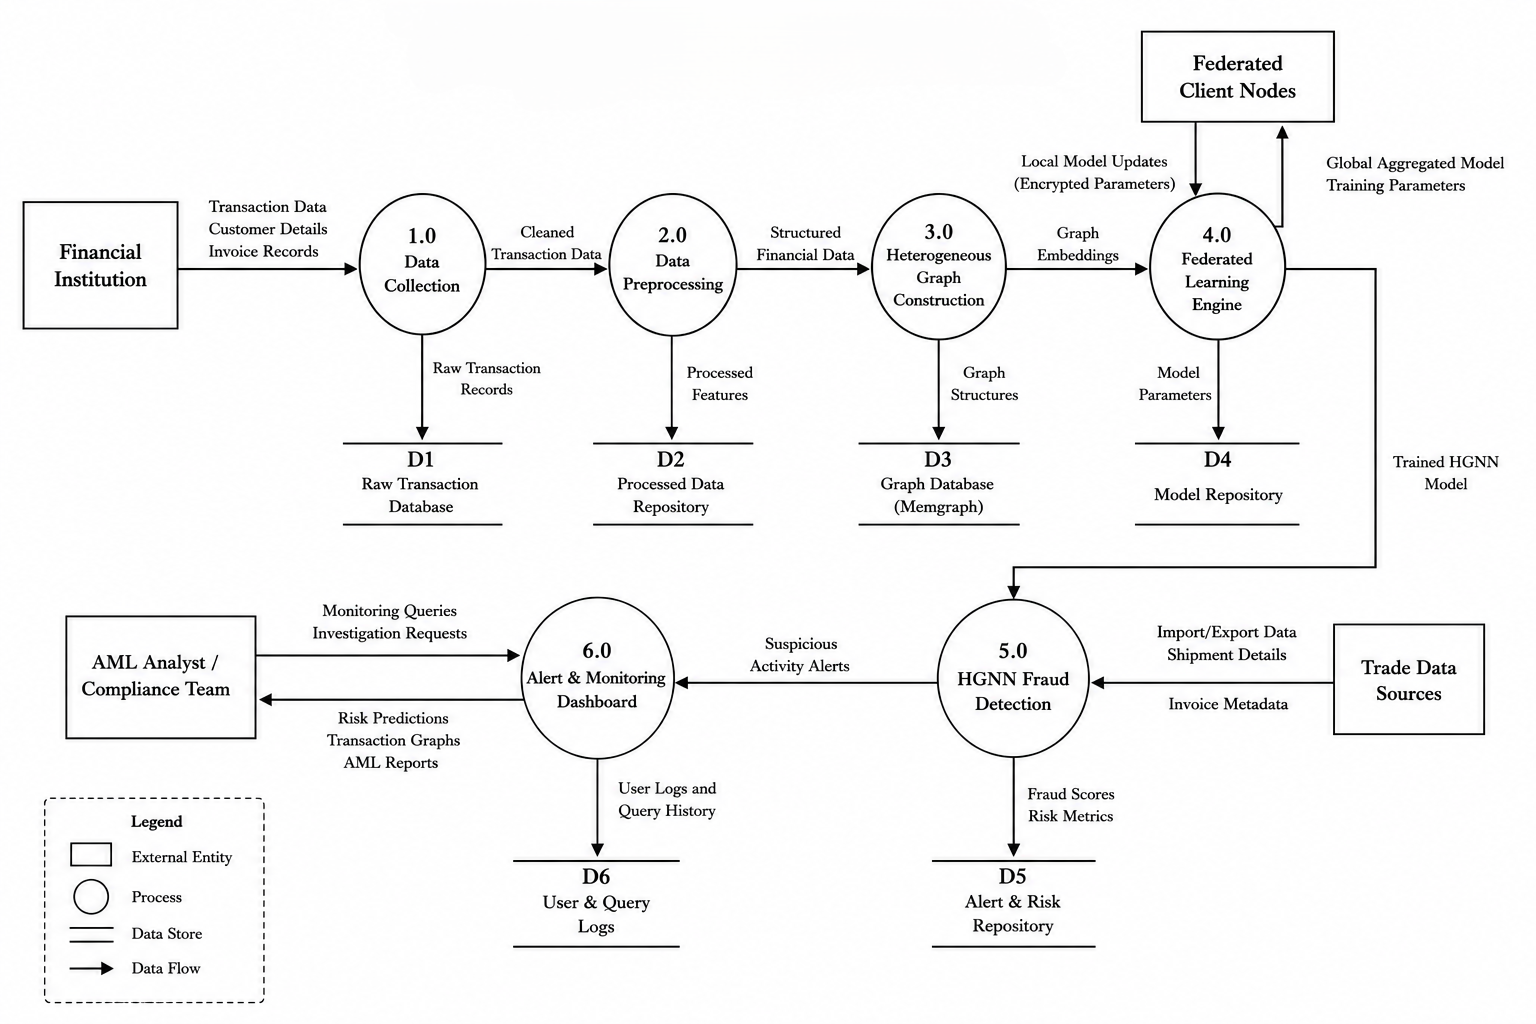
\includegraphics[width=\linewidth]{Figures/DFD_Level_1.png}
    \caption{Level 1 Data Flow Diagram}
    \label{fig:dfd_level1}
\end{figure}

The Level 1 Data Flow Diagram of the proposed TBML detection framework is shown in Figure \ref{fig:dfd_level1}. It breaks the main system into functional processes such as Data Collection, Data Preprocessing, Heterogeneous Graph Construction, Federated Learning Engine, HGNN Fraud Detection, and the Alert and Monitoring Dashboard. The Data Collection module gathers raw transactional data and customer data from financial institutions. That data is cleaned and transformed during preprocessing to produce structured financial features. Those features are then used by the graph construction engine to build heterogeneous graph representations stored in the graph database. The federated learning engine trains distributed collaborative models using encrypted local updates from federated client nodes while preserving institutional data privacy. The trained HGNN model is used by the fraud detection engine to identify suspicious transactional patterns, compute fraud scores, and generate anomaly alerts. Finally, the monitoring dashboard allows AML analysts and compliance teams to investigate cases, visualize transaction graphs, and review risk assessment reports in real time.
%========================================================
\subsubsection[Data Flow Diagram Level 2]{\textbf{Data Flow Diagram Level 2}}
%========================================================

\begin{figure}[H]
    \centering
    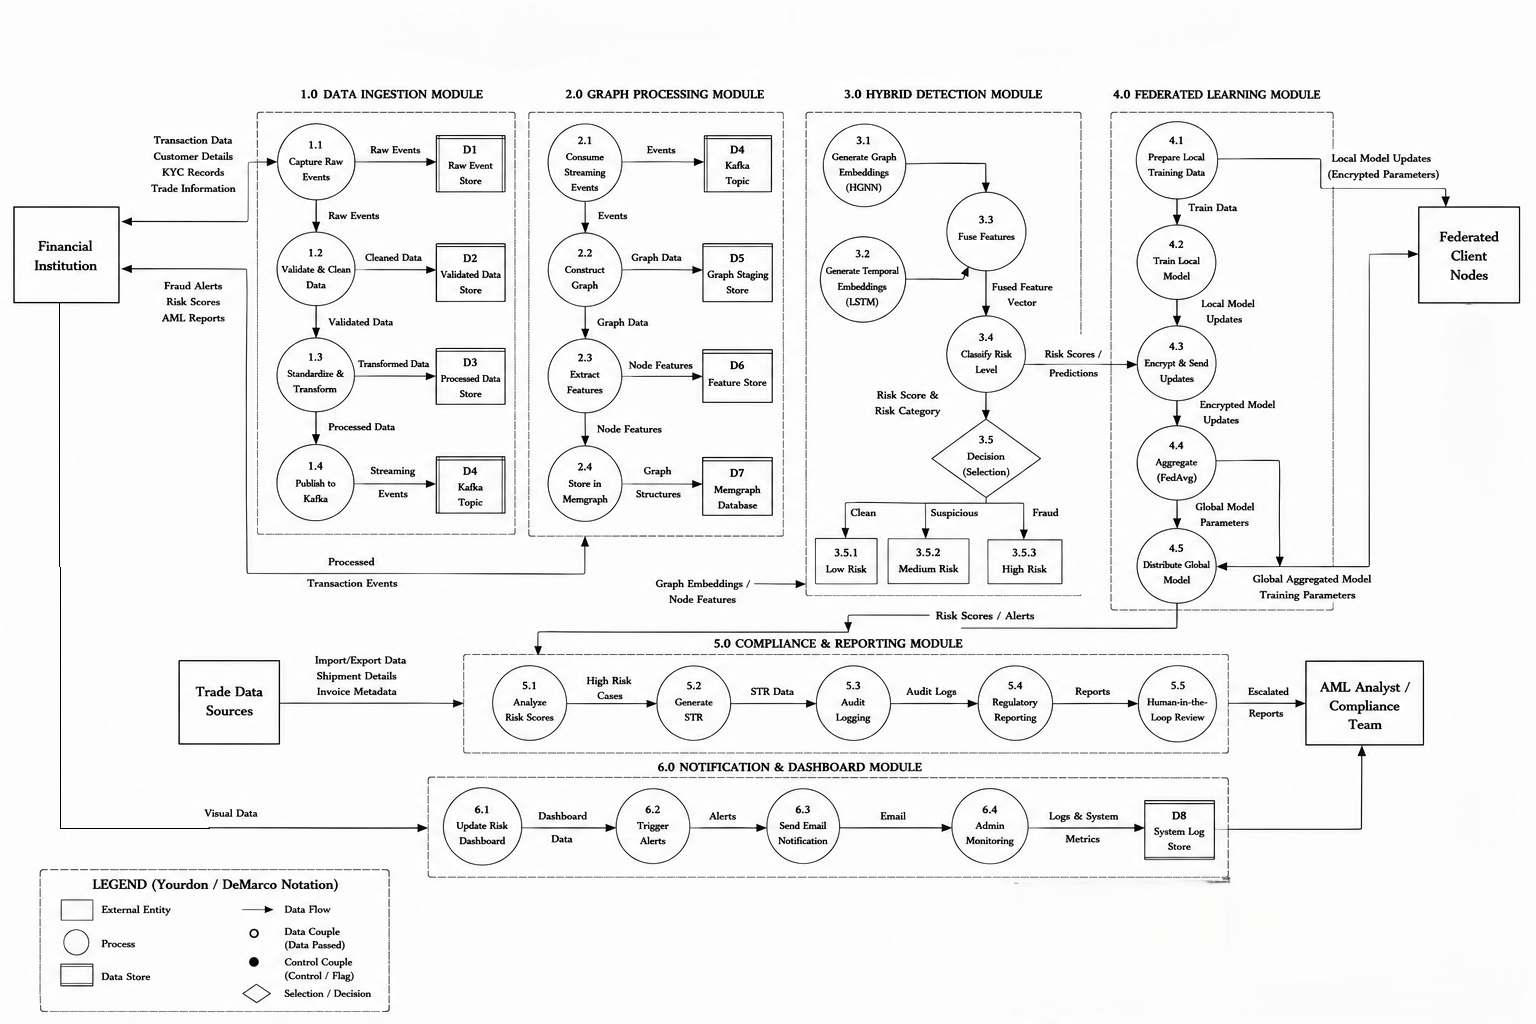
\includegraphics[width=\linewidth]{Figures/DFD_Level_2.png}
    \caption{Level 2 Data Flow Diagram}
    \label{fig:dfd_level2}
\end{figure}

Figure \ref{fig:dfd_level2} shows the Level 2 DFD, which breaks down the HGNN Fraud Detection module in more detail. The process begins with Data Integration and Validation, where trade invoice data, shipment data, and transactional metadata are checked for inconsistencies. After validation, the data moves into Entity Resolution and Feature Extraction, which handles attribute extraction and prepares the features needed for graph-based learning. Heterogeneous Graph Generation then builds the financial transaction graphs that connect entities, account relations, invoice transactions, and other trade-related structures. HGNN Inference and Risk Scoring applies the graph neural network to generate scores and identify suspicious transactional behavior. The results then move through Anomaly Detection and Classification, followed by Alert Generation and Prioritization, which ranks suspicious transactions according to risk. The final stage, Result Aggregation and Reporting, produces fraud summaries, alert notifications, and reports that are sent to the Alert and Monitoring Dashboard for review.


\section {Detailed System Design}
This section gives a detailed view of the system design for the proposed TBML detection framework. It covers the structure chart showing how the system components are organized, the functional descriptions of the major modules, and the interaction workflow between the services and analytical components in the framework.
%========================================================
\subsection[Structure Chart]{\textbf{Structure Chart}}
%========================================================
The structure chart of the proposed TBML detection framework shows how the key functional modules are arranged. The framework includes frontend, backend, fraud detection, federated learning, database, and compliance layers, all of which support scalable monitoring and intelligent fraud analysis in Anti-Money Laundering ecosystems.

The frontend layer provides dashboard interfaces, transaction monitoring, risk visualization, and STR management. The backend layer coordinates transactions between the frontend interface and the analytical modules by handling APIs, transaction management, authentication, and authorization. The fraud detection layer contains the Hybrid HGNN-LSTM modules that handle graph analytics, transaction analysis, feature fusion, and risk prediction.

The federated learning layer supports collaborative privacy-preserving model training and global model synchronization among participants. The database layer manages transactions, graphs, audit logs, and compliance data. The compliance layer handles STR generation, regulatory reporting, email notifications, and monitoring processes. The structural organization of the proposed TBML detection framework is shown in Figure~\ref{fig:structure_chart}.
\begin{figure}[H]
    \centering
    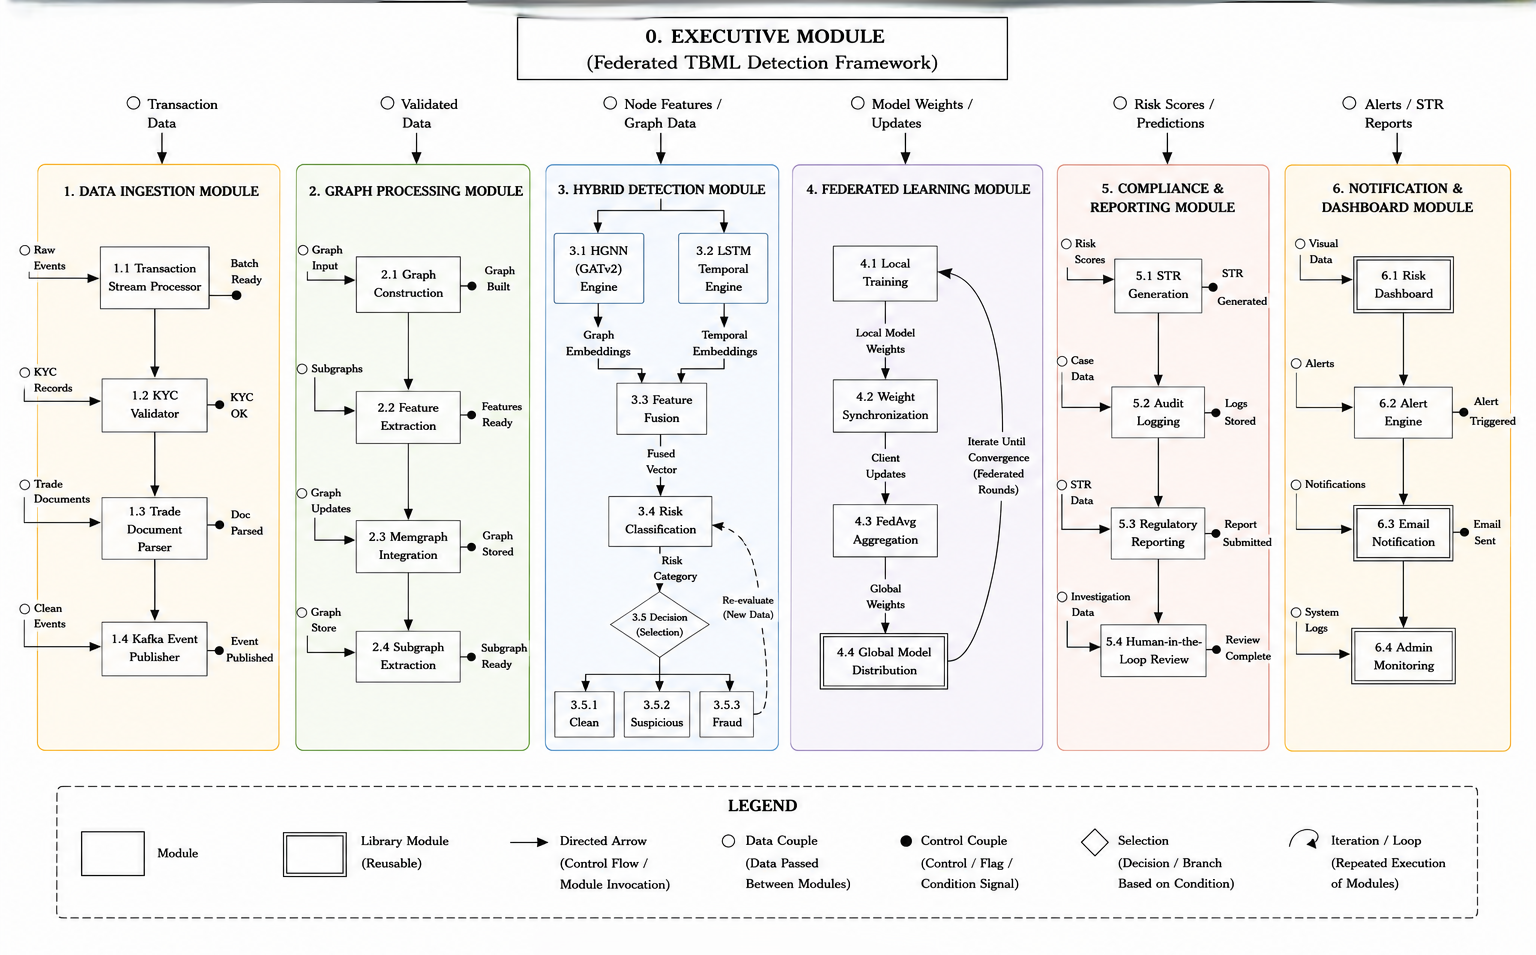
\includegraphics[width=\textwidth]{Figures/tbml_academic_structure_chart.png}
    \caption{Structure Chart of the Proposed TBML Detection Framework}
    \label{fig:structure_chart}
\end{figure}

The structure chart makes the modular organization of the framework easier to understand, especially the interaction between the analytical, monitoring, storage, and compliance-oriented services. This modular design improves scalability, maintainability, service integration, and coordination between the frontend interfaces, backend analytical services, and distributed fraud detection environments.

%========================================================
\subsection[Functional Description of the Modules]{\textbf{Functional Description of the Modules}}
%========================================================

The functional description of the modules explains the internal processing workflow and interaction between the major analytical, monitoring, and compliance-oriented components operating within the proposed TBML detection framework. The framework integrates transaction streaming services, graph construction mechanisms, hybrid HGNN--LSTM analytical models, institutional verification environments, and regulatory reporting systems to support intelligent Trade-Based Money Laundering detection and real-time compliance monitoring.

% %========================================================
% \subsection[Module Interaction Workflow]{\textbf{Module Interaction Workflow}}
% %========================================================

% The module interaction workflow shows how the main services of the proposed framework fit together, starting with transaction intake and ending with regulatory reporting. Financial transactions, KYC records, and trade documents first enter the transaction processing layer, where they are prepared and published to Kafka streaming topics for asynchronous communication between backend services.

% Kafka consumers read these transaction streams and pass the processed data to the graph construction and feature extraction module. Here, heterogeneous financial transaction graphs are built from accounts, transactions, trade entities, and document relationships stored in the Memgraph database. The resulting graph embeddings and relational features are then sent to the Hybrid HGNN--LSTM fraud detection module for graph representation learning, temporal transaction analysis, and fraud prediction.

% The fraud classifications and monitoring results produced by the analytical engine are stored in PostgreSQL and displayed in the dashboard environment for institutional investigators and banking administrators. Suspicious transactions are reviewed by authorized bank administrators and then marked as clean, suspicious, or confirmed fraudulent.

% Transactions confirmed as fraudulent are forwarded to the STR generation environment, where Suspicious Transaction Reports are prepared with support from the Groq API service. These reports are then reviewed by regulatory authorities responsible for investigation, inquiry, and enforcement. At the same time, notification management services coordinate fraud alerts and institutional communication, while the Resend email service delivers notification emails and regulatory messages to the relevant authorities. The overall module interaction workflow of the proposed TBML detection framework is illustrated in Figure~\ref{fig:workflow_interaction}.

\begin{figure}[H]
    \centering
    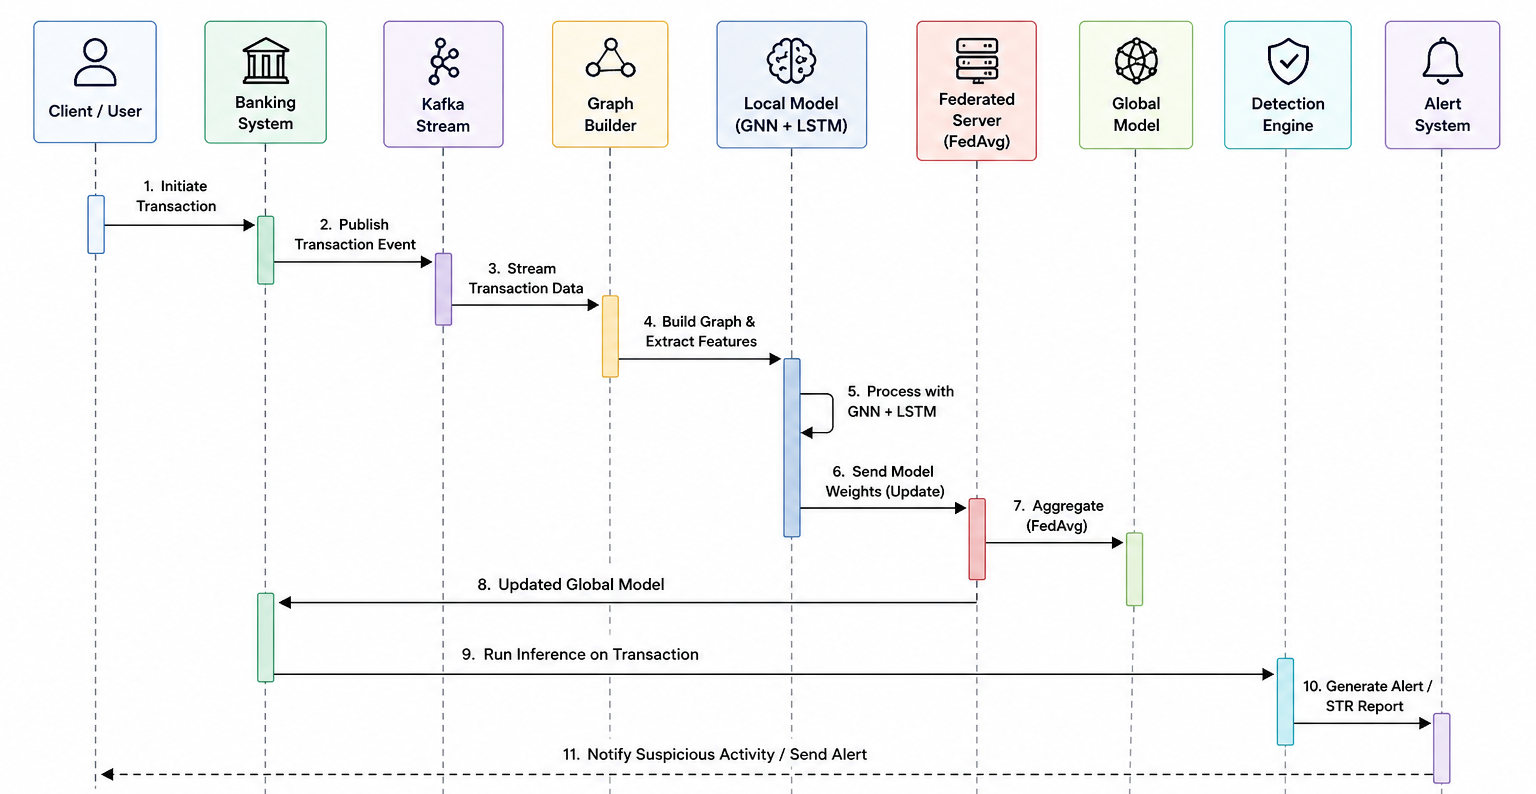
\includegraphics[width=\textwidth]{Figures/sequencediagramfinal.png}
    \caption{Workflow Interaction Diagram for the Proposed TBML Detection Framework}
    \label{fig:workflow_interaction}
\end{figure}

The workflow interaction diagram shows the coordinated interaction between streaming services, graph-based analytical modules, monitoring environments, institutional verification systems, and regulatory compliance services operating within the proposed framework. This modular workflow supports scalable transaction processing, intelligent fraud analysis, compliance management, and real-time Anti-Money Laundering monitoring across distributed financial environments.

%========================================================
\subsubsection[Transaction Processing Module]{\textbf{Transaction Processing Module}}
%========================================================

The transaction processing Module acts as the initial ingestion environment within the proposed TBML detection framework. This Module collects financial transactions, KYC records, trade documents, and institutional monitoring events originating from banking systems and external financial environments.

The input data processed within this Module includes sender and receiver account identifiers, transaction amounts, commodity types, trade quantities, trade values, invoice details, transaction timestamps, and institutional monitoring attributes associated with financial activities. The collected transactional data is validated, normalized, and converted into structured transaction records to support reliable downstream analytical processing.

The processed transaction events are published into Kafka streaming topics to enable asynchronous communication between backend services and analytical modules. The generated transaction streams serve as the primary input for graph construction, feature extraction, and graph-based fraud detection operations within the proposed framework.
%========================================================
\subsubsection[Graph Construction Module]{\textbf{Graph Construction Module}}
%========================================================

The graph construction module transforms processed transaction streams into heterogeneous financial transaction graphs for downstream graph-based analytical processing. The module receives validated transaction events from Kafka consumer services and models financial interactions between accounts, transactions, and trade documents within a connected graph environment.

The generated graph schema consists of interconnected node entities including \texttt{(:Account)}, \texttt{(:Transaction)}, and \texttt{(:Document)} connected through relationships such as \texttt{[:SENDS]}, \texttt{[:TO]}, and \texttt{[:HAS\_DOC]} as illustrated in Figure~\ref{fig:graph_schema}. The heterogeneous graph structure preserves transactional connectivity, intermediary account interactions, and trade-document relationships required for identifying hidden financial dependencies associated with Trade-Based Money Laundering activities.

The module interacts with the Memgraph database to store graph structures, entity relationships, and transactional connectivity information required for downstream feature extraction and fraud analysis. The generated graph representations and extracted relational features are subsequently forwarded to the Hybrid HGNN--LSTM fraud detection module for intelligent transaction classification.

\begin{figure}[H]
\centering

\begin{tikzpicture}[
    node distance=3cm,
    every node/.style={font=\scriptsize},
    entity/.style={
        draw=black,
        thick,
        rounded corners=8pt,
        align=center,
        minimum width=3cm,
        minimum height=2.2cm
    },
    relation/.style={
        -{Latex[length=2.5mm]},
        thick
    }
]

% ==========================================================
% ACCOUNT NODE
% ==========================================================

\node[
    entity,
    fill=orange!25
] (account)
{
\textbf{(:Account)}\\
\rule{2.2cm}{0.3pt}\\
account\_id\\
jurisdiction\\
is\_shell\\
dorm\_days
};

% ==========================================================
% TRANSACTION NODE
% ==========================================================

\node[
    entity,
    fill=red!20,
    right=of account
] (transaction)
{
\textbf{(:Transaction)}\\
\rule{2.2cm}{0.3pt}\\
txn\_id\\
amount\\
timestamp\\
risk\_score
};

% ==========================================================
% DOCUMENT NODE
% ==========================================================

\node[
    entity,
    fill=yellow!30,
    above=of transaction
] (document)
{
\textbf{(:Document)}\\
\rule{2.2cm}{0.3pt}\\
swift\_ref\\
price\_deviation\\
weight\_gap\\
commodity
};

% ==========================================================
% RELATIONSHIPS
% ==========================================================

\draw[relation]
(account) to[bend left=18]
node[midway, above] {\texttt{[:SENDS]}}
(transaction);

\draw[relation]
(transaction) to[bend left=18]
node[midway, below] {\texttt{[:TO]}}
(account);

\draw[relation]
(transaction) --
node[midway, right] {\texttt{[:HAS\_DOC]}}
(document);

\end{tikzpicture}

\caption{Heterogeneous graph schema representing entity attributes and transactional relationships in the proposed TBML detection framework.}

\label{fig:graph_schema}

\end{figure}


%========================================================
\subsubsection[Hybrid HGNN--LSTM Fraud Detection Module]{\textbf{Hybrid HGNN--LSTM Fraud Detection Module}}
%========================================================
The Hybrid HGNN--LSTM fraud detection module performs graph-based representation learning and temporal transaction analysis within the proposed TBML detection framework. The module receives KYC node features, graph edge relationships, SWIFT transaction attributes, sequential transaction tensors, and trade metadata extracted from the heterogeneous financial graph for downstream analytical processing.

The graph branch utilizes a three-layer GATv2 architecture to perform attention-based neighborhood aggregation and multi-hop message passing across interconnected financial entities. The stacked GATv2 layers improve two-hop neighborhood visibility and enable the model to capture hidden transactional relationships and intermediary account interactions associated with Trade-Based Money Laundering activities. The generated graph embeddings are globally pooled and fused with sequential transaction representations before being processed through the LSTM branch for temporal anomaly detection and transaction behavior analysis. In parallel, the trade branch processes trade-specific attributes including price deviation and weight gap scores using multilayer perceptron operations and feature normalization layers.

\begin{figure}[H]
    \centering
    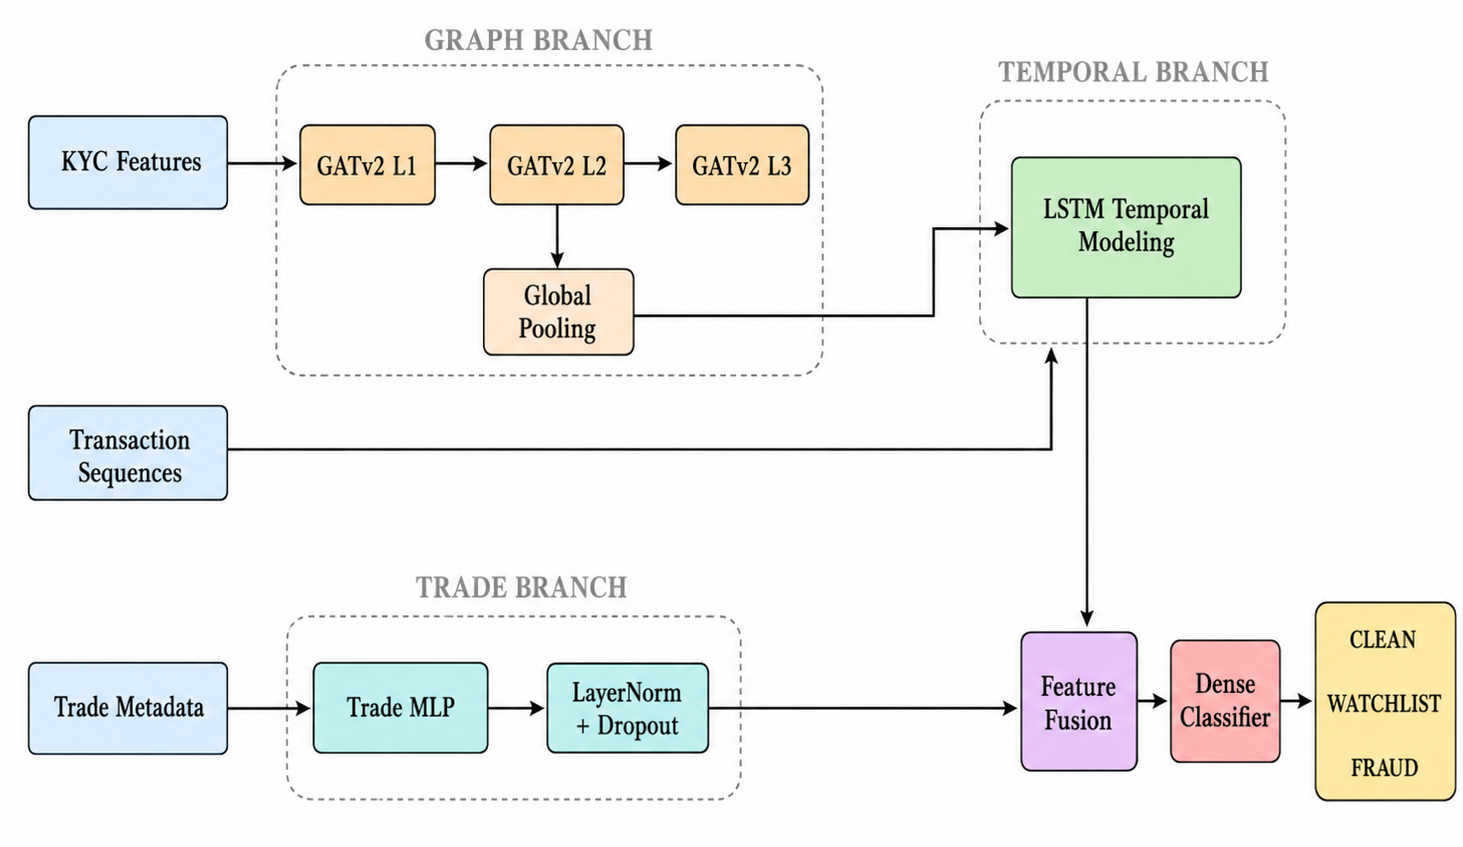
\includegraphics[width=\textwidth]{Figures/aimodel.png}
    \caption{Architecture of the Proposed Hybrid HGNN--LSTM Fraud Detection Module}
    \label{fig:hgnn_architecture}
\end{figure}

The generated graph embeddings, temporal representations, and trade feature vectors are combined within the feature fusion layer for downstream fraud prediction and transaction risk analysis. The final dense classification layer categorizes transactions into predefined classes including \texttt{CLEAN}, \texttt{WATCHLIST}, and \texttt{FRAUD}. The overall architecture of the proposed Hybrid HGNN--LSTM fraud detection module is illustrated in Figure~\ref{fig:hgnn_architecture}.

%========================================================
\subsubsection[Federated Learning Module]{\textbf{Federated Learning Module}}
%========================================================
The federated learning module enables privacy-preserving collaborative fraud detection across distributed financial institutions without directly sharing sensitive transactional data. Each participating institution performs local model training using institutional transaction graphs, transaction sequences, and fraud classification labels generated within the analytical environment. Independent federated clients maintain isolated training environments and perform localized optimization of the Hybrid HGNN--LSTM model on institution-specific financial datasets.

\begin{figure}[H]
    \centering
    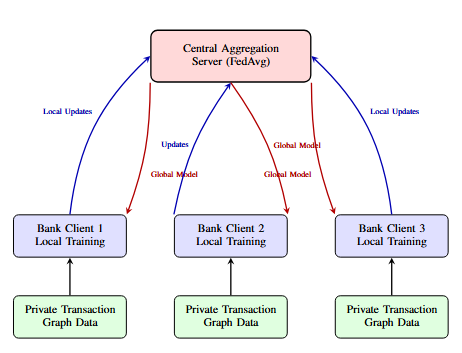
\includegraphics[width=0.82\textwidth]{Figures/federated_architecture.png}
    \caption{Federated learning architecture for privacy-preserving collaborative TBML detection across distributed institutions}
    \label{fig:federated_architecture}
\end{figure}

The framework utilizes the Federated Averaging (\texttt{FedAvg}) strategy to aggregate distributed model parameters across participating institutions. During each federated communication round, locally trained model weights generated from individual institutional clients are transmitted to the central aggregation server where parameter averaging operations are performed to generate a globally optimized fraud detection model. The aggregated global model parameters are subsequently redistributed to participating institutions for synchronized fraud detection and continuous real-time analytical inference. The overall federated learning architecture of the proposed framework is illustrated in Figure~\ref{fig:federated_architecture}.

%========================================================
\subsubsection[STR Generation and Notification Module]{\textbf{STR Generation and Notification Module}}
%========================================================

The STR generation and notification module is responsible for compliance reporting and fraud alert management within the proposed TBML detection framework. Transactions verified as fraudulent by authorized banking administrators are forwarded to this module for Suspicious Transaction Report (STR) generation and regulatory processing. The module generates STR reports containing transaction details, fraud classifications, trade metadata, institutional information, and investigation summaries associated with suspicious financial activities.

The Groq API service is utilized for analytical summarization and automated assistance during compliance documentation generation. Generated STR reports are subsequently forwarded to regulatory monitoring authorities for investigation and enforcement procedures. The notification management environment coordinates fraud alerts and institutional communication workflows, while the Resend email service delivers notification emails, investigation alerts, and regulatory enforcement messages to banking institutions and regulatory authorities.

%========================================================
\subsubsection[Dashboard and Regulatory Monitoring Module]{\textbf{Dashboard and Regulatory Monitoring Module}}
%========================================================

The dashboard and regulatory monitoring module provides real-time transaction visualization, fraud monitoring, and institutional investigation functionalities within the proposed TBML detection framework. The monitoring dashboard displays transaction classifications, fraud alerts, risk scores, STR records, and analytical monitoring information generated by the fraud detection environment. Separate dashboard environments are maintained for banking administrators and regulatory authorities to support institution-level monitoring and centralized compliance management operations.

For banking administrators, the dashboard provides a clear view of suspicious and fraudulent transactions flagged by the analytical model. They can review each case, verify the context, and then classify it as \texttt{CLEAN}, \texttt{WATCHLIST}, or \texttt{FRAUD}. This review step helps reduce false alarms while ensuring that genuine suspicious activity is escalated for further action. Transactions confirmed as fraudulent are then passed on for Suspicious Transaction Report (STR) generation and regulatory reporting.

Regulatory authorities use a separate monitoring view to track generated STR reports and institution-level fraud cases in one place. From this interface, they can follow compliance activity, request supporting documents, initiate inquiry procedures, and carry out account freeze operations when necessary. The overall workflow is illustrated in Figure~\ref{fig:realtime_workflow_final}.

\begin{figure}[H]
\centering
\resizebox{0.98\columnwidth}{!}{
\begin{tikzpicture}[
    node distance=1.1cm and 1.1cm,
    >=stealth,
    thick,
    every node/.style={font=\scriptsize},
    block/.style={
        draw,
        rectangle,
        rounded corners=3pt,
        align=center,
        minimum width=2.4cm,
        minimum height=0.9cm
    },
    storage/.style={
        draw,
        cylinder,
        shape border rotate=90,
        aspect=0.3,
        align=center,
        minimum height=1cm,
        minimum width=1.2cm
    }
]

\node[block, fill=blue!12] (txn) {Incoming\\Transactions};
\node[block, fill=orange!15, right=of txn] (kafka) {Kafka Streaming\\\& Graph Update};
\node[block, fill=green!15, right=of kafka] (model) {HGNN-LSTM\\Inference Model};
\node[block, fill=yellow!18, right=of model] (risk) {\texttt{CLEAN}\\ \texttt{WATCHLIST}\\ \texttt{FRAUD}};

\node[block, fill=cyan!15, below=1.8cm of model] (bank) {BankUser\\Dashboard};
\node[block, fill=red!15, left=of bank] (str) {STR Generation\\(GROQ LLaMA-70B)};
\node[block, fill=purple!15, right=of bank] (notify) {Email / Push\\Notification};

\node[block, fill=pink!18, below=1.8cm of notify] (admin) {Admin\\Dashboard};
\node[block, fill=orange!18, left=of admin] (action) {Freeze Account /\\Request Documents};

\node[storage, fill=gray!15] (db) at ($(action.west)-(2.2,0)$) {PostgreSQL};

\draw[->] (txn) -- (kafka);
\draw[->] (kafka) -- (model);
\draw[->] (model) -- (risk);

\draw[->] (risk.south) -- ++(0,-0.5) -| (bank.north);

\draw[->] (bank) -- (str);
\draw[->] (str.north) -- ++(0,0.4) -| (notify.north);
\draw[->] (notify) -- (admin);
\draw[->] (admin) -- (action);

\draw[->, dashed] (action.west) -- (db.east);
\draw[->, dashed] (str.south) |- (db.north);
\draw[<->, dashed] (bank.south) -- ++(0,-0.6) -| (db.north);
\draw[<->, dashed] (admin.south) |- ++(0,-0.5) -| (db.south);

\end{tikzpicture}
}
\caption{Real-time fraud inference and compliance workflow of the proposed TBML detection framework.}
\label{fig:realtime_workflow_final}
\end{figure}

%========================================================
\section[Summary]{\textbf{Summary}}
%========================================================

This chapter provided a detailed overview of the software specifications, architectural design, data flow diagrams, structure chart, and functional descriptions of the major modules in the proposed TBML detection framework. The discussion of the system architecture, module interactions, and analytical workflows gives a clearer picture of the operational mechanisms, service integration strategy, and real-time monitoring capabilities built into the framework for intelligent Trade-Based Money Laundering detection and compliance management across distributed financial environments.


